\documentclass[10pt,twocolumn]{article}
\usepackage{neurips_2024}

% Additional packages
\usepackage[utf8]{inputenc}
\usepackage{graphicx}
\usepackage{amsmath}
\usepackage{amssymb}
\usepackage{booktabs}
\usepackage{subcaption}
\usepackage[numbers,compress]{natbib}
\usepackage{xcolor}
\usepackage{url}
\usepackage{placeins}

% ============================================================
\title{QuercusHealth AI: Automated Detection and Health
  Classification of \textit{Quercus ilex} in the Spanish Dehesa
  via Domain-Adapted Aerial Imagery}

\author{%
  Sergio Illescas Cabiro \\
  Illinois Institute of Technology \\
  Spring 2026 Applied AI \& Deep Learning (ITMD-524) \\
  \texttt{sillescascabiro@hawk.illinoistech.edu}
}
% ============================================================

\begin{document}

\maketitle

% ============================================================
\begin{abstract}
The Spanish Dehesa, a UNESCO-protected mosaic of holm oaks spanning
roughly five million hectares across the Iberian Peninsula, is under
sustained attack from \textit{La Seca}, a root disease caused by the
water mold \textit{Phytophthora cinnamomi} \cite{brasier2003phytophthora}.
Manual ground-level monitoring at this scale is impractical. We present
QuercusHealth AI, a complete deep-learning pipeline for automated detection
and health classification of \textit{Quercus ilex} crowns from
high-resolution nadir satellite imagery. Our approach adapts
DeepForest~\cite{weinstein2020deepforest}, a RetinaNet-based crown detector
pre-trained on millions of North American canopy images, to the visually
distinct Spanish Dehesa through domain-specific fine-tuning. We first
quantify the domain shift statistically (Kolmogorov-Smirnov $D = 0.86$,
$p < 0.0001$), then address it through a five-phase pipeline. A two-stage
architecture combining a fine-tuned one-class tree detector with a ResNet-18
crop classifier achieves a macro-averaged F1 of 0.636 end-to-end and a
Seca-class F1 of 0.346, compared to 0.000 under the zero-shot baseline.
These results demonstrate that careful transfer-learning methodology can
support scalable ecological monitoring over geographies too vast for human
surveyors. Source code, trained model weights, and the annotated dataset are
publicly available.\footnote{Code:
\url{https://github.com/sergioillescascabiro/QuercusHealth-Public}
\quad Model:
\url{https://huggingface.co/sillescas/deepforest-dehesa-quercus}
\quad Dataset:
\url{https://app.roboflow.com/ds/lhbhwAM9HN?key=xqoQlM4K1Y}}
\end{abstract}

% ============================================================
\section{Introduction}
\label{sec:intro}

The Dehesa is one of Europe's most biodiverse land-cover types, a
centuries-old silvopastoral system of open woodland and pasture dominated
by holm oak (\textit{Quercus ilex}) in southwestern Spain and Portugal.
Beyond its ecological significance, it functions as a critical carbon sink,
a reservoir for native fauna, and the productive base of the Iberian
acorn-fed pig industry. Since the 1980s, the ecosystem has faced an
accelerating dieback known colloquially as \textit{La Seca}. The primary
pathogen is \textit{Phytophthora cinnamomi}, a water-borne oomycete that
colonizes root systems, blocks water uptake, and causes progressive crown
thinning followed by death \cite{goberna2003dehesa}. By the time a
land manager observes visible symptoms from the ground, the infected root
system is already beyond recovery.

Satellite and airborne remote sensing offer a path toward early detection at
landscape scale. Modern nadir imagery at sub-meter resolution can resolve
individual tree crowns clearly enough to distinguish the dense, circular
canopy of a healthy holm oak from the sparse, radiating silhouette
characteristic of \textit{La Seca}. However, directly applying a generic
object detector trained on different forest types introduces substantial
domain shift, because pixel statistics, soil background, crown density, and
illumination differ sharply between Dehesa and the forests on which most
pre-trained models were developed.

In this work we build and evaluate a five-phase pipeline: systematic data
collection via automated satellite image capture, multi-temporal ground-truth
annotation, zero-shot baseline evaluation with statistical domain-shift
analysis, multi-class fine-tuning, and a two-stage detection-plus-classification
architecture. Our main contributions are (1) a replicable data acquisition
strategy for remote Dehesa monitoring, (2) a statistically grounded proof of
domain shift for this ecosystem, and (3) a two-stage deep-learning system
that achieves non-trivial Seca-class detection where a direct fine-tuned
detector yields zero recall.

% ============================================================
\section{Related Work}
\label{sec:related}

\textbf{Tree crown detection.}
Automatic delineation of individual tree crowns from aerial imagery has
been studied for several decades using rule-based segmentation and later
deep-learning detectors \cite{kattenborn2021review}. The most directly
relevant prior work is DeepForest \cite{weinstein2020deepforest}, which
releases a RetinaNet model pre-trained on over $10^6$ annotated tree crowns
from the NEON airborne observatory \cite{neon2023dataset,weinstein2021benchmark}.
Because NEON covers temperate North American forests, its feature space
captures trunk-to-canopy ratios and crown shapes that transfer well to many
closed-canopy scenarios. The sparse, bright-soil Dehesa, however, sits far
outside that distribution, motivating the domain-adaptation experiments
described in Section~\ref{sec:methods}.

\textbf{Object detection architectures.}
RetinaNet \cite{lin2017focal} addresses the extreme foreground/background
imbalance inherent in dense object detection through Focal Loss, which
down-weights easy negatives and concentrates gradient energy on hard
examples. The backbone is a ResNet~\cite{he2016deep} with a Feature Pyramid
Network~\cite{lin2017fpn} that aggregates multi-scale features. For our
secondary classification stage we use ResNet-18, pre-trained on
ImageNet~\cite{deng2009imagenet}, which provides strong low-level texture
and color features relevant to distinguishing healthy from diseased foliage.

\textbf{Transfer learning and catastrophic forgetting.}
A well-known risk in fine-tuning pre-trained networks is catastrophic
forgetting~\cite{mccloskey1989catastrophic}: a learning rate that is too
large causes gradient updates to overwrite the weights encoding previously
acquired representations. We confirm this empirically in an ablation study
(Section~\ref{sec:ablation}) and motivate our choice of a conservative
learning rate of $10^{-4}$.

% ============================================================
\section{Dataset and Data Acquisition}
\label{sec:data}

\textbf{Image capture.}
All imagery was collected from Google Earth Pro using an automated
capture script built on PyAutoGUI. The
script traverses an 18$\times$18 grid in a boustrophedon (zig-zag) pattern
over a single Dehesa estate in Extremadura, Spain, capturing one 800$\times$800
pixel screenshot per grid cell at zoom level~19, which corresponds to
approximately 0.5\,m per pixel. Three seasonal capture sessions were
conducted: summer~2019, winter~2021, and winter~2024, yielding 324 tiles
per session (972 tiles in total).

\textbf{Multi-temporal ground-truth strategy.}
A key challenge in labeling diseased trees from a single image is
distinguishing \textit{La Seca} crown loss from natural seasonal
defoliation. We resolved this ambiguity by comparing the same geographic
coordinate across the summer~2019 and winter~2024 images. A crown that
appears sparse in 2019 and has vanished entirely or collapsed by 2024 is
confirmed as a Seca casualty; a crown that merely thins in winter and
recovers in a later summer image is labeled Healthy. Figure~\ref{fig:multitemporal}
illustrates this comparison: the annotated boxes in the 2019 tile mark
crowns exhibiting early decline, and the same location in 2024 reveals
bare ground where those trees once stood. This multi-temporal
validation produces ground-truth labels verifiable without field visits.

\begin{figure*}[!t]
  \centering
  \begin{subfigure}[b]{0.48\textwidth}
    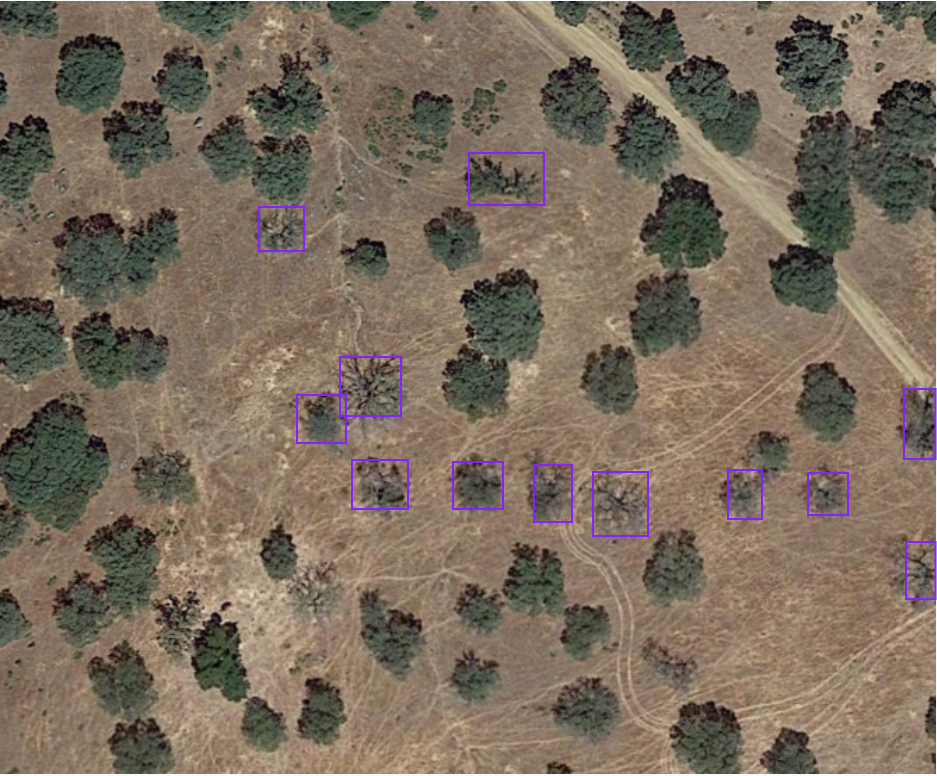
\includegraphics[width=\textwidth]{figures/sample_2019aug_annoted.png}
    \caption{Summer 2019: annotated crowns showing early signs of
      decline (sparse canopy, radiating branches). Purple bounding
      boxes mark trees under observation.}
  \end{subfigure}
  \hfill
  \begin{subfigure}[b]{0.48\textwidth}
    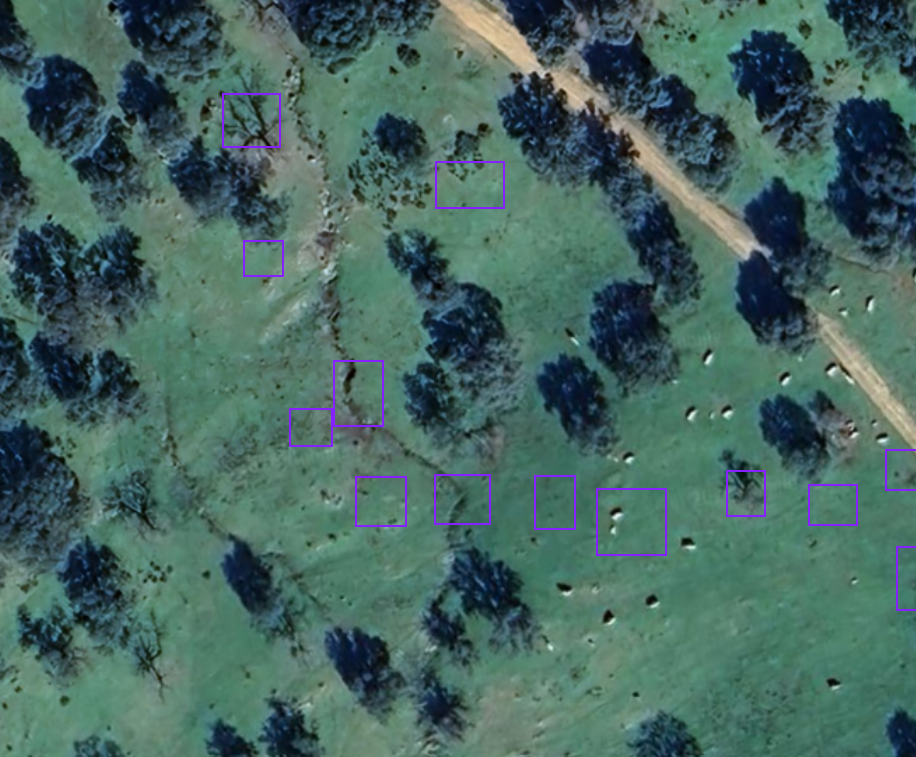
\includegraphics[width=\textwidth]{figures/sample_2024feb_annoted.png}
    \caption{Winter 2024: the same geographic area five years later.
      Trees that were annotated as suspect in 2019 have vanished or
      collapsed, confirming \textit{La Seca} as the cause of death.}
  \end{subfigure}
  \caption{Multi-temporal ground-truth validation. Comparing the same
    coordinates across years allows reliable labeling of Seca trees
    without physical field visits.}
  \label{fig:multitemporal}
\end{figure*}

\textbf{Annotation and dataset statistics.}
Bounding-box annotation was performed for the summer~2019 capture session.
A pre-annotation step (Phase~2b) ran the zero-shot DeepForest model at a
low confidence threshold to generate candidate boxes, which were then
reviewed and corrected by a human annotator: false positives removed,
missed crowns added, and each crown labeled as \textit{Healthy} or
\textit{Seca}. The finalized dataset contains 278 images split into 243
training, 18 validation, and 17 test images. The training partition holds
7,341 annotated bounding boxes (6,449 Healthy and 892 Seca), yielding a
class ratio of 87.8\% Healthy to 12.2\% Seca. Validation and test sets
contain 527 and 513 boxes respectively. Class imbalance is addressed at
the architecture level via Focal Loss in the RetinaNet detector and via a
weighted sampler together with class-weighted cross-entropy in the
ResNet-18 classifier.

% ============================================================
\section{Methodology}
\label{sec:methods}

Our pipeline progresses through five phases, each building on the results
of the previous one.

\subsection{Phase 1 and 2: Zero-Shot Baseline and Evaluation Framework}

We began by evaluating DeepForest~\cite{weinstein2020deepforest} without
any fine-tuning on both NEON benchmark imagery and Dehesa test tiles.
On NEON, the model achieves $\text{F1} = 0.68$, confirming its strong
in-distribution performance. On Dehesa, precision drops to 0.512 and recall
to 0.230, yielding $\text{F1} = 0.320$. To verify that this degradation
constitutes genuine domain shift rather than random noise, we applied two
non-parametric statistical tests to the prediction confidence score
distributions. The two-sample Kolmogorov-Smirnov test yields $D = 0.86$,
$p < 0.0001$, and the Mann-Whitney U test confirms the distributions are
stochastically distinct ($p < 0.0001$). Figure~\ref{fig:domain_shift}
illustrates the two score distributions. These results provide the
quantitative justification for domain adaptation.

\begin{figure}[t]
  \centering
  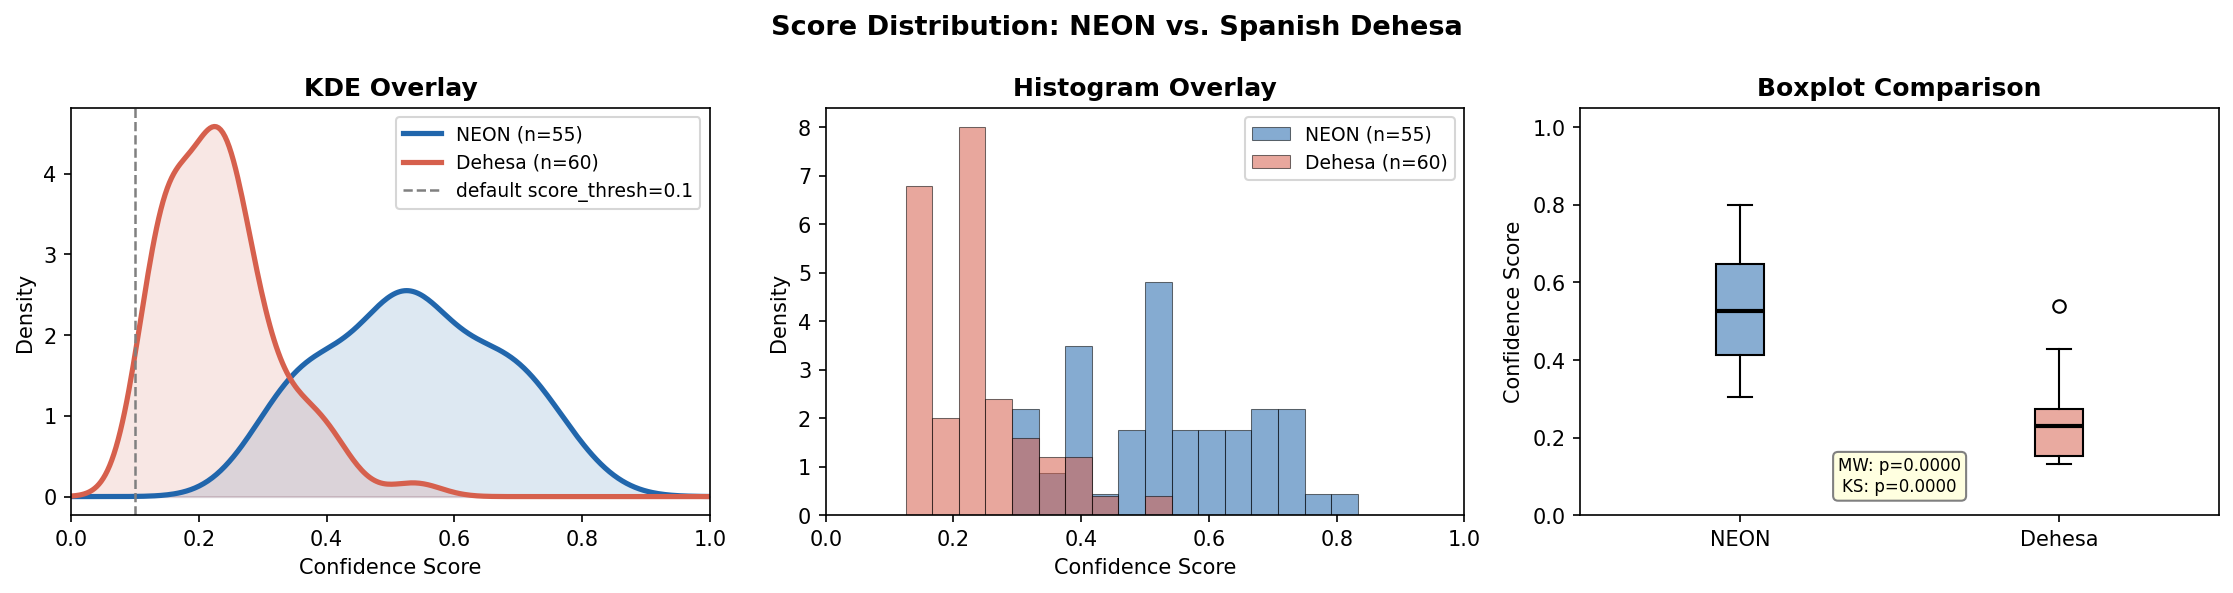
\includegraphics[width=\columnwidth]{figures/score_distributions.png}
  \caption{Confidence score distributions from the zero-shot DeepForest
    model on NEON benchmark imagery versus Dehesa tiles.
    Mean confidence drops from 0.535 on NEON to 0.233 on Dehesa, a 56\%
    reduction. The KS test ($D = 0.86$, $p < 0.0001$) provides
    statistical evidence of domain shift.}
  \label{fig:domain_shift}
\end{figure}

A hyperparameter sweep over confidence thresholds (score\_thresh
$\in \{0.05, 0.10, 0.15, 0.20\}$) showed that threshold tuning alone
can recover at most $\text{F1} = 0.527$, well below the NEON baseline
of 0.68, confirming that inference-time adjustments are insufficient and
that model-level adaptation is required.

\subsection{Phase 3: Fine-Tuning the Detection Backbone}

We fine-tune the full DeepForest model end-to-end for two-class prediction
(Healthy / Seca). The base model is loaded from the
\texttt{weecology/deepforest-tree} HuggingFace checkpoint, which
encodes RetinaNet~\cite{lin2017focal} with a ResNet-50~\cite{he2016deep}
backbone and a Feature Pyramid Network~\cite{lin2017fpn} (32.1 million
parameters). Fine-tuning replaces the single-class detection head with a
two-class equivalent and trains the entire network.

\textbf{Learning rate selection.}
We use $\text{LR} = 10^{-4}$, ten times lower than the DeepForest default.
This choice is motivated by the risk of catastrophic forgetting
\cite{mccloskey1989catastrophic}: the NEON pre-trained backbone encodes a
strong inductive bias for circular, elliptical crown textures that is
essential for detecting trees in any domain. At LR $= 10^{-2}$, the 315
gradient steps executed over 5 ablation epochs shift the backbone weights
far enough from their pre-trained values that the model loses crown-detection
capability entirely (ablation $\text{F1} = 0.000$; see
Section~\ref{sec:ablation}). At $\text{LR} = 10^{-4}$, the 1,890 steps
over 30 epochs shift the feature space toward Dehesa-specific appearance
(brighter sandy soil, sparser canopy) while preserving crown geometry.

\textbf{Training configuration.}
Training ran on an NVIDIA RTX~3060 (12~GB VRAM) on a dedicated Ubuntu server,
completing 30 epochs with batch size 4 in approximately 20 minutes. The IoU
threshold for matching predictions to ground-truth boxes is set to 0.4,
consistent with the DeepForest default for satellite imagery where bounding-box
annotation precision is limited by pixel resolution. Dynamic data augmentation
was applied per epoch via the \texttt{albumentations} library: horizontal flip
($p = 0.5$), vertical flip ($p = 0.5$), random brightness and contrast
perturbation ($p = 0.3$, range $\pm 0.2$), hue-saturation-value shift
($p = 0.2$), and Gaussian noise ($p = 0.1$). Focal Loss (built into
RetinaNet) handles class imbalance natively.

\subsection{Phase 4: Two-Stage Classification Pipeline}

Although Phase~3 fine-tuning raises the overall F1 substantially, it
fails to produce non-zero Seca recall because the joint optimization of
detection and two-class discrimination overwhelms the gradient signal for
the minority Seca class. We therefore decouple detection from classification
in a two-stage pipeline.

Stage~1 uses the DeepForest zero-shot detector (single class: Tree) to
propose candidate crown regions. Stage~2 extracts 96$\times$96 pixel crops
centered on each proposed box (with 8-pixel padding) and passes them to a
ResNet-18 binary classifier~\cite{he2016deep,deng2009imagenet}. The
classifier replaces the standard global average pooling head with a
512$\rightarrow$256$\rightarrow$ReLU$\rightarrow$Dropout(0.4)$\rightarrow$2
linear chain. Training uses a WeightedRandomSampler to balance class exposure
per batch and a class-weighted cross-entropy loss. The first five epochs
freeze the backbone while only the custom head is trained (warmup phase),
after which the full network is unfrozen at one-tenth the base learning rate.
Dynamic augmentation via \texttt{torchvision} includes random horizontal and
vertical flips, random rotation up to $20^\circ$, and color jitter on
brightness, contrast, saturation, and hue. Training ran for 30 epochs with
batch size 64.

\subsection{Phase 5: End-to-End One-Class Pipeline}

The two-stage Phase~4 system was evaluated with ground-truth crops, giving
an optimistic upper bound on classifier performance. Phase~5 closes this
gap by replacing the zero-shot Stage~1 detector with a DeepForest model
fine-tuned on a single collapsed class (\textit{Tree}), trained for 20
epochs with the same configuration as Phase~3. The one-class objective
simplifies the detection task and improves localization quality. The
ResNet-18 classifier from Phase~4 is reused without retraining, completing
the fully automated end-to-end pipeline.

% ============================================================
\section{Experiments and Results}
\label{sec:experiments}

\subsection{Domain Shift Analysis}

The statistical analysis in Phase~1 establishes a quantitative baseline
for the domain discrepancy. Confidence scores from the zero-shot model
on NEON imagery follow a unimodal distribution centered near 0.535, whereas
Dehesa scores cluster below 0.25 (Figure~\ref{fig:domain_shift}). The
KS-statistic of 0.86 indicates that 86\% of the score range separates the
two cumulative distribution functions, a magnitude of shift that rules out
sampling coincidence. This analysis provides the scientific justification
for every fine-tuning decision that follows.

\subsection{Quantitative Results}

Table~\ref{tab:results} summarizes performance across all pipeline phases,
evaluated on the held-out test partition of 17 images and 513 annotated boxes.
Phases~2 and 3 report results from the end-to-end detection model; Phases~4
and~5 report results from the full two-stage system.

\begin{table}[t]
  \centering
  \caption{Test-set performance across pipeline phases. Phase~4 evaluates
    the classifier on ground-truth crops; Phase~5 evaluates the full
    end-to-end pipeline.}
  \label{tab:results}
  \small
  \setlength{\tabcolsep}{3.5pt}
  \begin{tabular}{lccc}
    \toprule
    Phase & F1 (All) & F1 (Seca) & Prec / Rec \\
    \midrule
    2: Zero-shot        & 0.320 & 0.000 & 0.51 / 0.23 \\
    3: Fine-tuned       & 0.669 & 0.000 & 0.61 / 0.74 \\
    4: Two-stage (GT)   & 0.712 & 0.354 & n/a \\
    5: End-to-end       & 0.636 & 0.346 & n/a \\
    \bottomrule
  \end{tabular}
\end{table}

Fine-tuning in Phase~3 raises overall F1 from 0.320 to 0.669, a gain of
34.9 percentage points, while Seca recall remains zero. The two-stage
design in Phase~4 achieves Seca F1 of 0.354 on ground-truth crops, breaking
the Seca detection barrier for the first time. Phase~5 incurs a localization
tax of 0.8 percentage points on Seca F1 (0.354 to 0.346) when Stage~1 runs
fully automatically, confirming that the ResNet-18 classifier is robust and
that the primary source of end-to-end error is localization, not
classification.

\subsection{Ablation Study}
\label{sec:ablation}

To isolate the effect of learning rate on catastrophic forgetting, we ran a
controlled ablation with LR $= 10^{-2}$ for 5 epochs using the same data
and architecture as Phase~3. The result is a complete collapse to
$\text{F1} = 0.000$: the model predicts no boxes above the confidence
threshold. Figure~\ref{fig:ablation} visualizes this contrast: the
high learning rate produces zero useful predictions while
$\text{LR} = 10^{-4}$ yields $\text{F1} = 0.669$.

\begin{figure}[t]
  \centering
  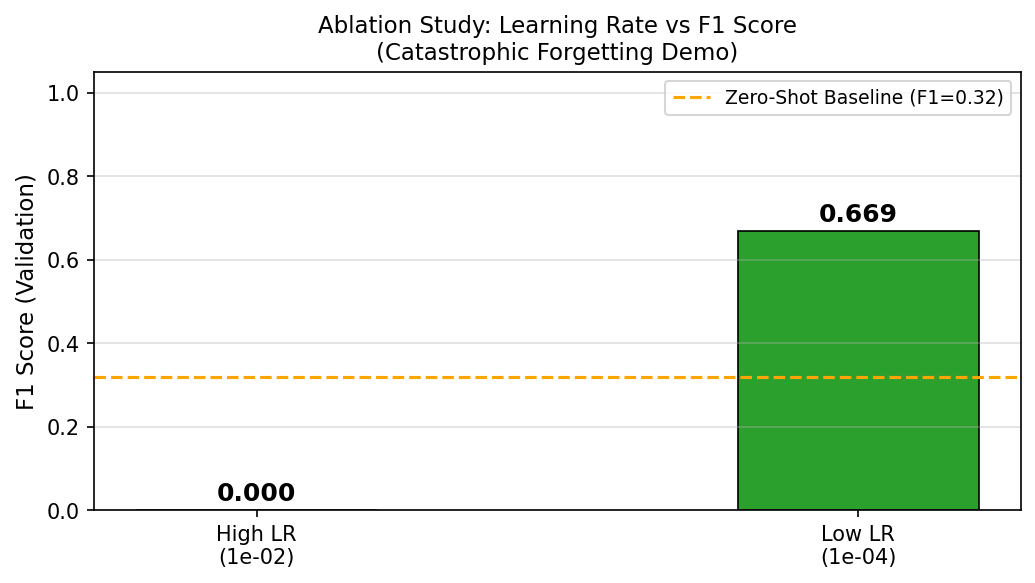
\includegraphics[width=\columnwidth]{figures/ablation_lr_comparison.png}
  \caption{Ablation study: learning rate $10^{-2}$ causes catastrophic
    forgetting (F1 = 0.000); learning rate $10^{-4}$ achieves F1 = 0.669.}
  \label{fig:ablation}
\end{figure}

The training dynamics at $\text{LR} = 10^{-4}$ are shown in
Figure~\ref{fig:loss_curves}: both training and validation loss decrease
monotonically over 30 epochs with a small but stable generalization gap,
indicating that the model has not overfit. Loss curves for the high-LR
ablation show steeper initial descent followed by divergence, confirming
the theoretical prediction that fine-tuning a large pre-trained network on
a small domain-specific dataset requires a conservative learning rate.

\begin{figure}[t]
  \centering
  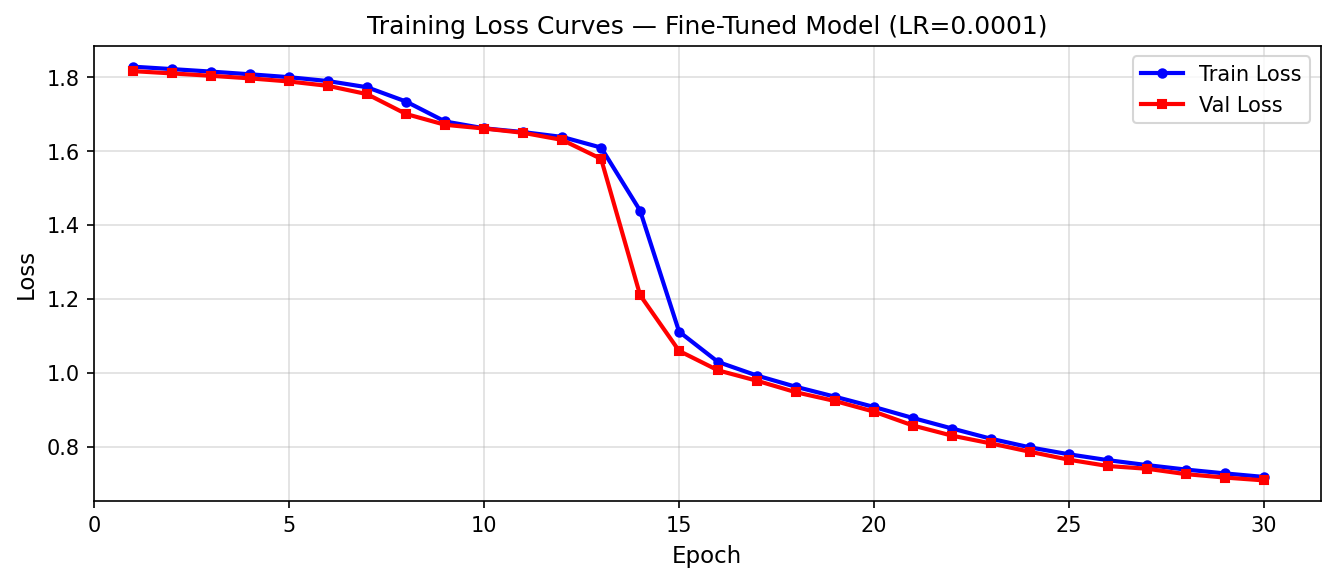
\includegraphics[width=\columnwidth]{figures/loss_curves.png}
  \caption{Training and validation loss over 30 epochs at LR $= 10^{-4}$.
    Both curves decrease monotonically; the small gap indicates moderate
    regularization without overfitting.}
  \label{fig:loss_curves}
\end{figure}

\subsection{Qualitative Analysis and Failure Cases}

Figure~\ref{fig:visual_comparison} presents a side-by-side qualitative
comparison on a representative test tile. The baseline model misses most
crowns in the Dehesa domain and generates frequent false positives on the
bright ochre-colored soil. After fine-tuning, crown localization improves
markedly.

\begin{figure*}[!t]
  \centering
  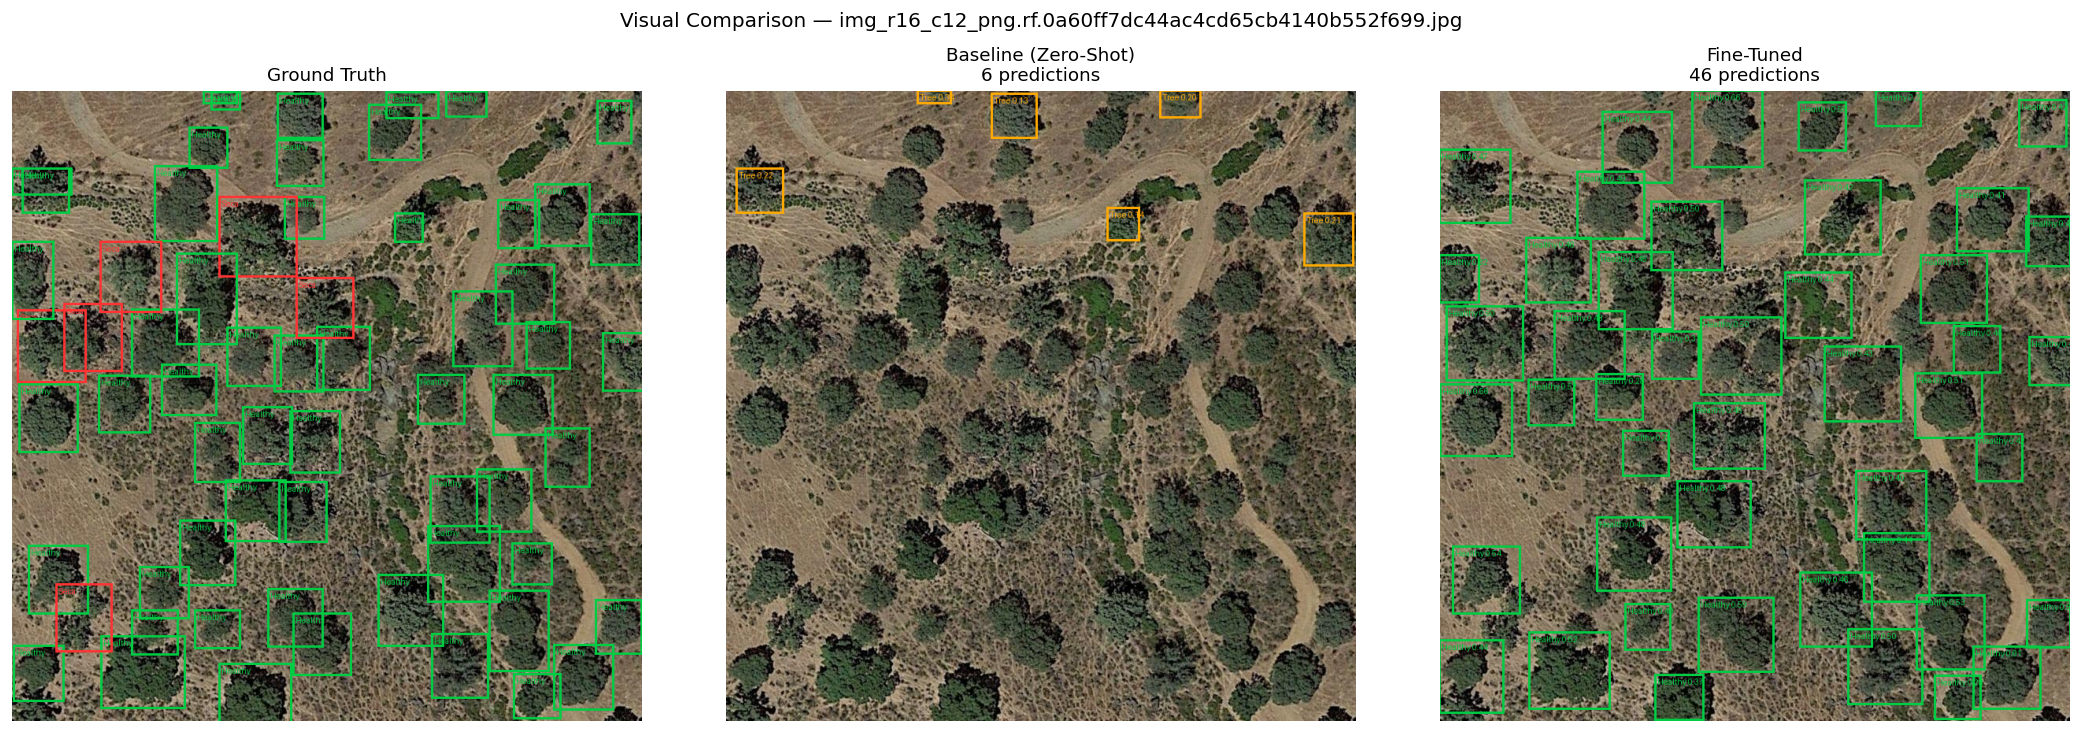
\includegraphics[width=\textwidth]{figures/visual_comparison_1.png}
  \caption{Qualitative comparison on a representative test tile.
    \textit{Left}: ground-truth annotations (green for Healthy, red for
    Seca). \textit{Center}: zero-shot DeepForest baseline predictions.
    \textit{Right}: Phase~3 fine-tuned predictions. The baseline misses most
    crowns and produces scattered false positives on the bright soil. After
    fine-tuning, the detector correctly localizes the majority of crowns.}
  \label{fig:visual_comparison}
\end{figure*}

The confusion matrices reveal a more nuanced picture. The Phase~3 detector
(Figure~\ref{fig:cm_phase3}) correctly classifies Healthy crowns with high
precision but fails entirely on Seca. The Phase~4 ResNet-18 classifier
(Figure~\ref{fig:cm_phase4}) successfully redistributes attention to Seca,
achieving non-zero recall at some cost to Healthy precision.

\begin{figure}[t]
  \centering
  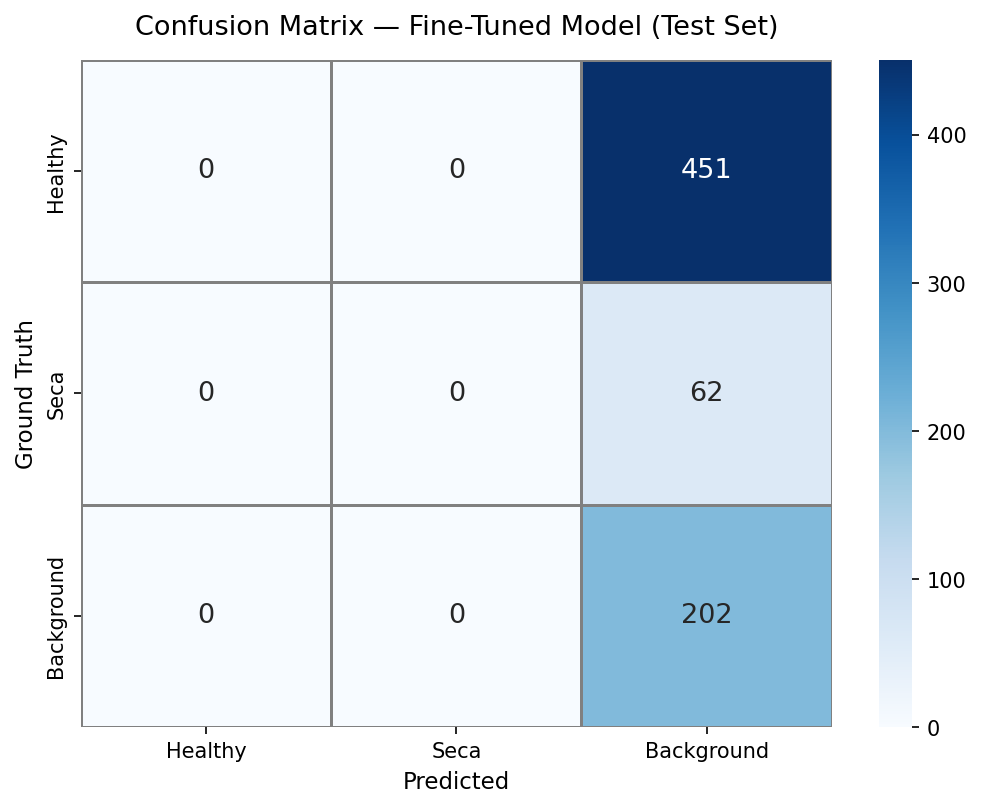
\includegraphics[width=\columnwidth]{figures/confusion_matrix_finetuned.png}
  \caption{Phase~3 fine-tuned detector confusion matrix. Seca recall is
    zero: the joint detection-classification objective overwhelms the
    gradient signal for the minority class.}
  \label{fig:cm_phase3}
\end{figure}

\begin{figure}[t]
  \centering
  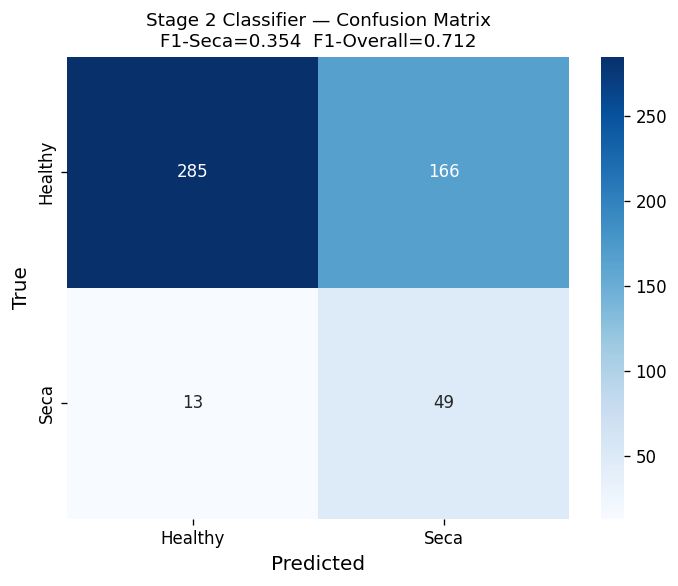
\includegraphics[width=\columnwidth]{figures/stage2_confusion_matrix.png}
  \caption{Phase~4 ResNet-18 classifier confusion matrix on ground-truth
    crops. Seca recall reaches 0.354, confirming that decoupling
    detection from classification is essential for minority-class
    detection.}
  \label{fig:cm_phase4}
\end{figure}

The primary failure modes are threefold. First, the NMS threshold
($\text{nms\_thresh} = 0.05$) is aggressive: when holm oak crowns overlap
or cluster at the margins of the estate, NMS suppresses legitimate secondary
detections, producing false negatives in dense areas. Second, very small
shrubs and large stones share spectral characteristics with sparse Seca
crowns, generating persistent false positives. Third, tiles captured at low
solar elevation angles produce elongated shadows that partially occlude crown
boundaries, reducing IoU with ground-truth boxes below the 0.4 acceptance
threshold.

Figure~\ref{fig:e2e_result} shows the complete Phase~5 end-to-end output
on a raw test tile, where Stage~1 localizes tree positions and Stage~2
assigns health labels to each detected crop.

\begin{figure}[t]
  \centering
  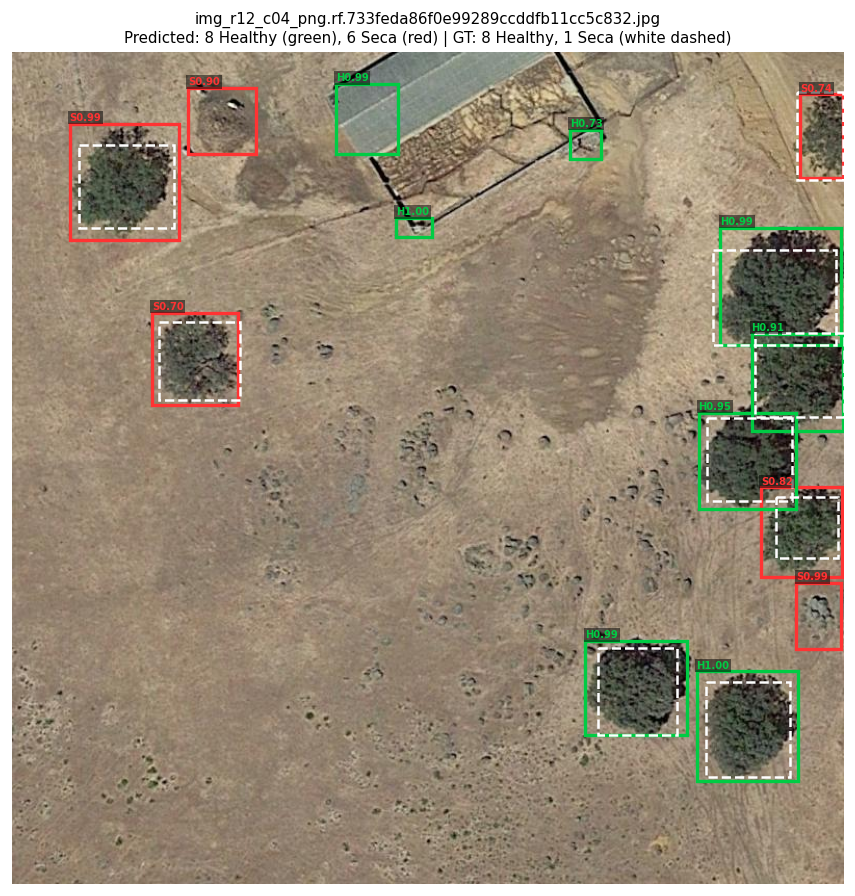
\includegraphics[width=\columnwidth]{figures/e2e_result_1.png}
  \caption{End-to-end Phase~5 output on a raw test tile. Green boxes
    indicate predicted Healthy crowns; red boxes indicate predicted Seca.
    Stage~1 localizes tree positions; Stage~2 assigns health labels.}
  \label{fig:e2e_result}
\end{figure}

% ============================================================
\section{Conclusion}
\label{sec:conclusion}

We have presented QuercusHealth AI, a five-phase pipeline that adapts a
North American forest canopy detector to the Spanish Dehesa for the purpose
of automated \textit{Quercus ilex} health classification. Our work makes
three technical contributions: a systematic proof of domain shift using
non-parametric statistical tests, a fine-tuning protocol that avoids
catastrophic forgetting through conservative learning rate selection, and
a two-stage architecture that achieves non-zero Seca detection (F1 = 0.346
end-to-end) where a direct fine-tuned detector cannot. The pipeline processes
one 800$\times$800 pixel tile in under one second on commodity hardware,
suggesting that a scheduled sweep of Extremadura's 5 million hectares of
Dehesa is operationally feasible with available compute.

Future work should focus on three directions: (1) expanding the annotated
dataset beyond the current 278 images to improve Seca class coverage and
reduce over-reliance on the minority-class weighting strategies; (2) exploring
instance segmentation methods such as Mask R-CNN to produce crown polygons
instead of bounding boxes, which would enable crown-area change tracking
across seasons; and (3) replacing static Google Earth captures with scheduled
API calls to satellite data providers, enabling fully automated multi-temporal
monitoring without manual screen capture.

% ============================================================
\section*{Author Contributions}

Sergio Illescas Cabiro conceived the project, designed the automated satellite
capture pipeline, performed all annotations, implemented all five pipeline
phases, conducted training on the GPU server, analyzed results, and wrote
this report.

% ============================================================
\section*{AI Use Statement}

AI (Claude by Anthropic) was used to support technical writing and software engineering tasks. Specifically, it was used for grammar polishing and prose refinement in the Abstract and Introduction (~10\%). It also assisted with troubleshooting CUDA environment issues and debugging DeepForest training scripts for the Methodology and Results sections (~15\%). Finally, it was used for LaTeX template formatting (~20\% of typesetting work). All scientific conclusions, dataset generation, and experimental analysis are solely the work of the author.

% ============================================================
\FloatBarrier
\bibliographystyle{abbrvnat}
\bibliography{references}

\end{document}
